\section{Introduction}
\subsection{Outline}

\begin{frame}
  \begin{center}
    {\large Lecture 02 -- Data Structures\\Part I -- Introduction}\\
  \end{center}
\end{frame}

\begin{frame}
  \frametitle{Outline}

  When writing any program (and not just programming challenges!) the right data structure makes a great difference in \structure{how easy the program is to write} and \structure{how time and memory efficient the algorithm is}.\bigskip

  \begin{itemize}
    \item In this lecture, we will review some data structures that commonly appear in programming challenges;\medskip

    \item This lecture covers Chapter 2 of the "Competitive Programming" book;\medskip

    \item In this lecture, we focus the {\bf description and implementation} of data structures more than on their theoretical analysis.
  \end{itemize}
\end{frame}

\begin{frame}
  \frametitle{Comments on the last week:}

  \begin{itemize}
    \item Numbers of Problems solved;\medskip

    \item Orders of Problems;\medskip

    \item Lecture Calendar for this week;
  \end{itemize}
  \vfill

  \begin{block}{Motivating Problems}
    To introduce the topics of this class, let's show three problems where the choice of data structure can make a big difference;
  \end{block}
\end{frame}

\subsection{Motivating Problems}


\begin{frame}[fragile]
  \frametitle{Example 1: 8 Queen Problem (UVA 750)}
  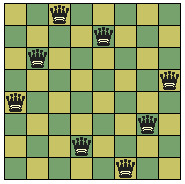
\includegraphics[width=0.25\textwidth]{../img/8queen}\\
  \ppagenote{Chessboard by Lee Daniel Crocker. CC-BY-SA 3.0}

  For a board of size $n \times n$, you have to find \alert{how many} safe
  configurations of $n$ queens exist.
  \bigskip

  Because you need to count \alert{how many} configurations exist, it is
  necessary to test {\bf all} valid configurations.

  \bigskip

\begin{verbatim}
for (int i = 0; i < #configurations; i++)
  if configurationIsSafe(i) sum++
return(sum)
\end{verbatim}
\end{frame}

\begin{frame}[fragile]
  \frametitle{Example 1: 8 Queen Problem (UVA 750)}

  Last lecture we talked about how {\bf pruning} can be used to reduce the problem size. This time we review this concept more concretely.\bigskip

  Consider how we store information about all the configurations. Imagine that we have an array, \emph{conf}, which contains all configurations that we want to test.
  \bigskip

  Approach 1: For each queen, we store the pair $(\text{col},\text{row})$.
\begin{verbatim}
conf[0]   = {{a,1}, {a,1}, {a,1}, ... {a,1}, {a,1}}
conf[1]   = {{a,1}, {a,1}, {a,1}, ... {a,1}, {a,2}}
conf[2]   = {{a,1}, {a,1}, {a,1}, ... {a,1}, {a,3}}
  ...
conf[k]   = {{a,1}, {b,2}, {b,2}, ... {c,8}, {d,8}}
conf[k+1] = {{a,1}, {b,2}, {b,2}, ... {c,8}, {e,1}}
  ...
\end{verbatim}

Looping through all options: $n^{n^2}$ steps
\end{frame}

\begin{frame}[fragile]
  \frametitle{Example 1: 8 Queen Problem (UVA 750)}
  Approach 2: We fix each queen on a column (a,b,c,d...). Our data structure only needs to represent the row of each queen. \bigskip

  We store an array of arrays, containing 8 integers representing the row:\bigskip
\begin{verbatim}
conf[0]   = {0,0,0,0,0,0,0,0}
conf[1]   = {0,0,0,0,0,0,0,1}
conf[2]   = {0,0,0,0,0,0,0,2}
  ...
conf[k]   = {0,0,0,3,3,6,7,7}
conf[k+1] = {0,0,0,3,3,7,0,0}
  ...
\end{verbatim}
Looping through all options: $n^n$ steps
\end{frame}

\begin{frame}[fragile]
  \frametitle{Example 1: 8 Queen Problem (UVA 750)}
  Approach 3: We fix each queen on a column (a,b,c,d...), and each configuration
  is a permutation of rows where we place the queens. \bigskip

  We store a string of rows, and each configuration is a permutation accessed using "next\_permutation" function from C++ stl's "algorithm" header. \bigskip

\begin{verbatim}
conf[0] = "01234567"
conf[1] = "01234576"
conf[2] = "01234657"
  ...
\end{verbatim}
\end{frame}

\begin{frame}
  \frametitle{Example 2: The Towers of Hanoi}

  \begin{center}
    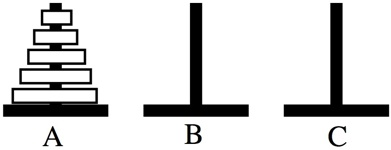
\includegraphics[width=0.5\textwidth]{img/hanoi}
  \end{center}
  \medskip

  {\small
    \begin{itemize}
    \item You have $N$ disks and $K$ poles. Each disk has unique size $s_i$.
    \item A disk $i$ can be moved from one pole to another.
    \item A move of disk $i$ to pole $k$ is only valid if $k$ has no disks smaller than $i$
    \item Find the list of moves to move all disks from pole 1 to pole $K$.
    \end{itemize}
  }

  \vfill

  How do you represent the data in this problem?
\end{frame}

\begin{frame}
  \frametitle{Example 2: The Towers of Hanoi}
  A string with ``n'' disks, from smaller to larger.
  \begin{center}
    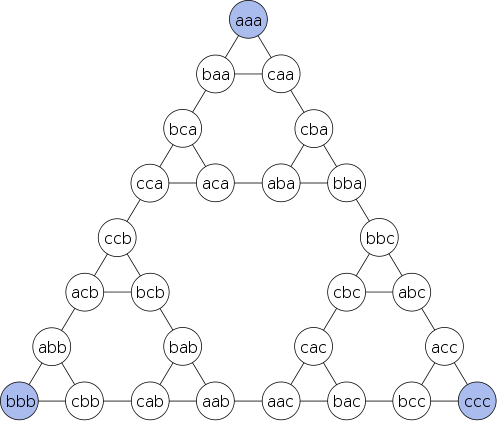
\includegraphics[width=0.65\textwidth]{img/hanoi_graph}
  \end{center}
  \ppagenote{Tower of Hanoi's graph image by nonenmac}
\end{frame}

\begin{frame}[fragile]
  \frametitle{Example 3: Army Buddies (UVA 12356)}
  \framesubtitle{Problem Description}

  \begin{block}{}
    \begin{itemize}
    \item There is a line of $S$ soldiers: $0,1,2,3,4,...,S$
    \item There are $Q$ queries that remove soldiers from $i$ to $j$:
\begin{verbatim}
Q1: 2,4           (removes soldiers 2, 3, 4)
Q2: 6,7           (removes soldiers 6, 7)
Q3: 1,1           (removes soldier 1)
\end{verbatim}
    \item For each query, list the soldier to the \alert{left} and to the \alert{right}
\begin{verbatim}
A1: 1,5       1 x x x 5 6 7
A2: 5,*       1 - - - 5 x x
A3: *,5       x - - - 5 - -
\end{verbatim}
    \end{itemize}
  \end{block}

  \bigskip

  How do we solve this problem?
\end{frame}

\begin{frame}
  \frametitle{Example 2: Army Buddies (UVA 12356)}
  \framesubtitle{Idea 1: Linked Lists}

  \begin{columns}
    \column{0.5\textwidth}
    For each query, we find the first soldier, and we remove each soldier
    until we find the second soldier.\bigskip

    We use the linked list to reduce the size of the list after each query.
    \column{0.5\textwidth}
    \begin{center}
      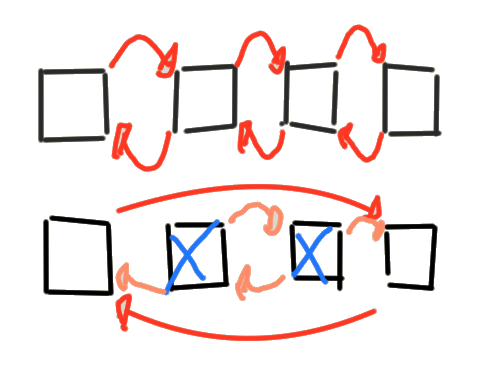
\includegraphics[width=1\textwidth]{img/army-list}
    \end{center}
  \end{columns}

  \begin{itemize}
  \item Represent the line as a linked list.
  \item Find the 1\textsuperscript{st} soldier and 2\textsuperscript{nd} soldiers \hfill \structure{($O(n)$ steps)}
  \item Repeat the operation above for each query. \hfill \structure{($O(nm)$ steps)}
  \end{itemize}
  \bigskip

\end{frame}

\begin{frame}
  \frametitle{Example 2: Army Buddies (UVA 12356)}
  \framesubtitle{A solution using linked lists}

  \begin{center}
    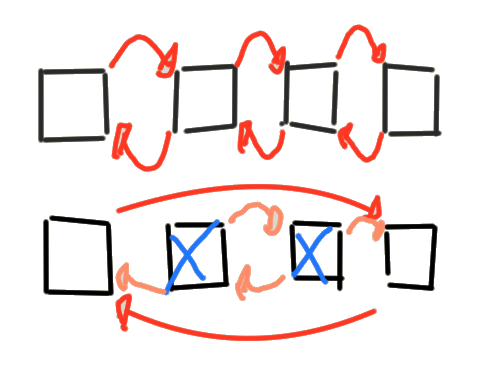
\includegraphics[width=0.4\textwidth]{img/army-list}
  \end{center}

  \alert{Problem!} The input is too big, and $O(nm)$ takes too much time.

  \begin{itemize}
  \item $1 \leq S \leq B \leq 10^5$;\hfill \structure{($O(10^5\times 10^5)) = 10^{10}$}
  \item Also \alert{multiple cases};\hfill \structure{($O(n^2k)) = 10^{10}k$}
  \end{itemize}

  \bigskip

  Let's think of a different solution! (Before looking at the next slide)
\end{frame}


\begin{frame}[t]
  \frametitle{Example 2: Army Buddies (UVA 12356)}
  \framesubtitle{A solution using arrays}

  The problem with last solution is that it costs $n$ to search the soldiers. We need to access the sodier position in $O(1)$ using an {\bf index}. We also need to keep track of neighbors when removing soldiers.

  \begin{itemize}
  \item \alert{Idea}: To use {\bf two} Neighbor Arrays
    \begin{itemize}
    \item Let {\bf R} be: {\bf Int} Array of Right neighbors
    \item Let {\bf L} be: {\bf Int} Array of Left neighbors
      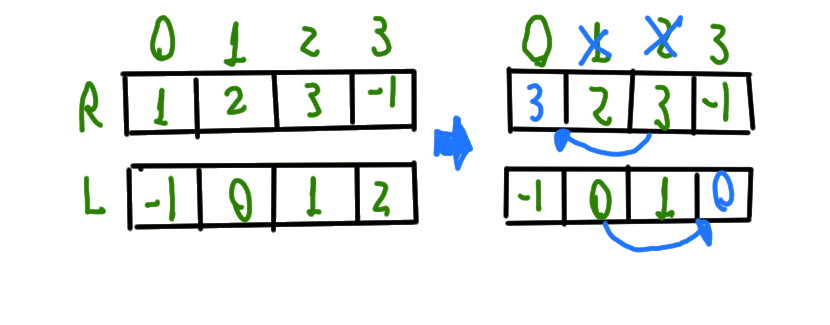
\includegraphics[width=0.7\textwidth]{img/army-array}
    \end{itemize}
  \item \alert{Question}: how do we update R and L after query $(r,l)$?\\
  \end{itemize}
\end{frame}

\subsection{Thinking about Data Structures}
\begin{frame}{Motivating Data Structure}
  As you can see, the choice of data structure and problem representation is very important.\bigskip

  \begin{itemize}
    \item Choosing the right data structure:
    \begin{itemize}
      \item Changes the time or memory complexity of the implementation;
      \item Makes the programming task simpler or more complex;
    \end{itemize}\medskip

    \item Hints for programming contests;
    \begin{itemize}
      \item Avoid using pointers (source of bugs, programming overhead);
      \item Prefer multiple variables, instead of complex structs;
      \item In larger programs (not challenges) you want more complex structures;
    \end{itemize}\medskip

    \item Learn the library tools of your language (STL, java.utils, etc);
  \end{itemize}\bigskip

  \hfill {\bf End of part I}
\end{frame}
